\section{Malware Information Retrieval System}
In this section, we describe the behavior, configuration, and properties of the proposed malware retrieval system. Our system is divided into two phases: training and retrieval. During the training phase, we train the representation vectors of the training data that reflect the semantics. During the retrieval phase, the ranking result is output from the query from the user. The following subsections define the notations to be used in the two phases and use them to describe in detail which tasks to perform in each phase.

\subsection{Notations}
We have $X = \{x_1, x_2, ..., x_N\}$ as a training malware set. We also have a multi-label set, $Y = \{\mathbf{y}_{1}, \mathbf{y}_{2}, ... , \mathbf{y}_{N}\}$, corresponding to malware labels. Then, $V = \{v_1, v_2, ..., v_n \}$ is defined as a set of hand-crafted features extracted from malware.

MR system is defined as tuple with $[u, h, E, d, R]$ elements. $u$ is a feature extractor module that extracts the hand-crafted features from malware sample. $h$ is an embedding function that obtains a representation vector from malware features. $E$ is the embedded representation vector set of malwares to be retrieved. $d$ is a function that calculates the distance between the input query and the embedded representation vector. $R$ is a ranking module. %During the training phase, it learns the appropriate $h$ and gets $E$ from $V$. During the retrieval phase, the malware sample query, $q$, is entered, and the nearest $k$ neighbors are returned via the ranking module, $R$.


\begin{table}[!htb] % notation
\caption{List of Symbols}
\label{tab:notation}
\begin{minipage}{\columnwidth}
\begin{center}
\begin{tabular}{ll}
\toprule
Symbol & Meaning\\
\midrule
  $X$ & Set of malwares \\
  $x_i$ & i-th malware sample \\
  $v_i$ & Extracted features of i-th malware\\
  $V$ & Set of extracted features \\
  $Y$ & Set of multi-labels  \\
  $\mathbf{y}_{i}$ & Multi-labels of i-th malware\\
  $u$ & Feature extractor \\
  $h$ & Neural embedder \\
  $\theta$ & Parameters of neural embedder \\
  $g$ & Classifier \\   
  $W$, $\mathbf{b}$ & Parameters of classifier \\  
  $E$ & Set of embedded malware representation vectors \\
  $\mathbf{e}$ & Embedded malware represnetation vector \\
  $\mathbf{c}$ & Importance coefficient \\
  $d$ & Distance measuring function \\
  $S$ & Set of semantic component vectors \\
  $\mathbf{s_i}$ & i-th semantic component vector \\
  $R$ & Ranking module \\
  $\mathbf{e}_q$ & Embedded representation vector of queried sample \\
  
\bottomrule
\end{tabular}
\end{center}
\bigskip\centering
\end{minipage}
\end{table}


\subsection{Tasks}
During the training phase, to obtain represenation vectors used in MR system, we perform an auxiliary task to classify supervised labels. The auxiliary task can be a single label classification or a multi-label classification. $f: V \rightarrow Y $ f is a function that estimates a label from malware features. The function, $f$, can be defined as a composite function of $g$ and $h$. $h$ is an embedding function for obtaining representation vectors from the malware features described above. $g$ is a classifier that can estimate labels from representation vectors. 
\[
f(v_i) = (g \circ h)(v_i) = g(h(v_i)) = g(\mathbf{e_i}) = y_i 
\]
where
\[
g(\mathbf{e_i}) = \sigma (W\mathbf{e_i} + \mathbf{b}) 
\]

See Section 4 for details on how to train representation vectors that contain semantics.
 
% sigma == sigmoid or softmax
In the retrieval phase, the malware sample query, $q$, is embedded using the h function that already trained at training phase. The distance between the representation vector of the query, $\mathbf{e_q}$ and stored represenation vectors $E$, is measured through the $d$ function, and the nearest $k$ samples are returned through the ranking module, $R$.

\begin{figure}[!htb] % train_phase
  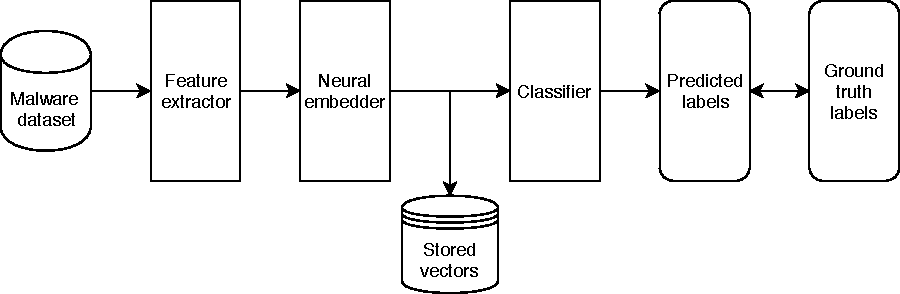
\includegraphics[width=\linewidth]{../../figures/train_phase.pdf}
  \caption{The structure to perform training phase.}
  \label{fig:train_phase}
\end{figure}

\begin{figure}[!htb] % retrieval_phase
  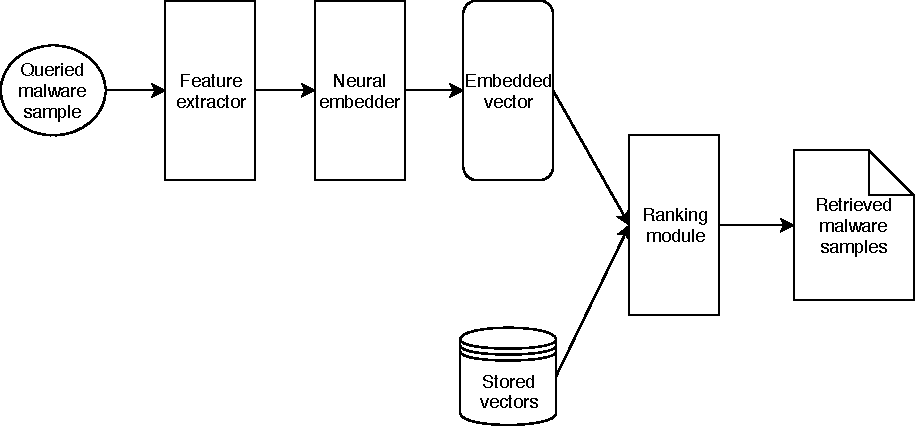
\includegraphics[width=\linewidth]{../../figures/retrieval_phase.pdf}
  \caption{The structure to perform retrieval phase.}
  \label{fig:retrieval_phase}
\end{figure}


\subsection{Modules}
The structure of the two phases is shown in the Figure.\ref{fig:train_phase} and Figure.\ref{fig:retrieval_phase}. The common modules in both phases include the feature extractor and the neural embedder. The training phase includes the classifier, and the retrieval phase contains the ranking module.

\textbf{Feature extractor. }
The feature extractor is a module that extracts hand-crafted features from raw malware sample. For example, hand-crafted features, such as size, entropy, and histogram-of-API-calls can be extracted. In the case of APK, an additional permission feature can be extracted. 

\textbf{Neural embedder. }
The neural embedder creates a vector representation from the features of malware extracted from the feature extractor module. This is a neural network parameterized with $\theta$, and parameters are optimized while performing the auxiliary task in the training phase. During the retrieval phase, the parameters are not updated. 

\textbf{Classifier. }
The classifier module represents the probability that the sample corresponds to each label based on the vector representations from the neural embedder. It is parameterized in one fully connected layer and it uses softmax or sigmoid activation depending on the task. Like the neural embedder module, the parameters are trained by back-propagation in the training phase and not updated in the retrieval phase.

\textbf{Ranking module. }
We measure the distance between the vector representations obtained from the input sample, and the embedding vectors of the training data set using the distance function, d, and output nearest k samples.


\subsection{Desired Properties}
Extant MR systems have limitations. They could not retrieve samples that have similar meanings with different structure. It also fails to cope with the emerging variants and new families. To become a MR system that solves this problem, the following attributes must be satisfied.

\textbf{Semantic understanding. }
The system should be able to rank and retrieve not only structurally similar samples but also semantically similar samples for the input query. Even if the structure of two malwares is different, both have the same meaning if the behavior of the malwares are the same. Likewise, if the behavior is quite different, even if it is structurally nearly the same, the two samples will have different meanings. For example, we think that the similarity of samples between \texttt{ransomware} families, \texttt{locky} and \texttt{cerber}, is smaller than the similarity between the two samples of different family, \texttt{locky} and \texttt{coinminer} even though they are more structurally similar. Also if the semantic difference like having a same variant type or adding a same malicious action is preserved for specific samples, the it could be called as semantics-aware system.
 
\textbf{Robustness to novel samples. }
New malware variants continue to appear and the system must respond quickly.

\textbf{Efficiency. }
A large number of malware currently exist. Thus, to retrieve the k-ranked results of many samples in a reasonable time, the ranking module should be efficient.


